This section describes the Control Unit layer, responsible for processing input data, managing system logic, and generating output signals.
\begin{figure}[h!]
	\centering
 	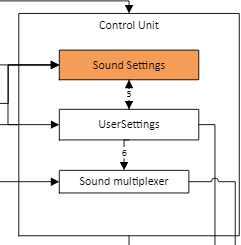
\includegraphics[width=0.60\textwidth]{images/SoundSettings.png}
 \caption{Sound Settings subsystem description diagram}
\end{figure}
\subsection{Sound setting}
This section describes the Control Unit layer, responsible for processing input data, managing system logic, and generating output signals.


\subsubsection{Assumptions}
The Sound Settings subsystem receives digital signals from the UserSettings and the Sound Settings subsystem is responsible for managing and applying the sound settings based on user input.

\subsubsection{Responsibilities}
\begin{itemize}
\begin{item}
Receive digital signals from the UserSettings subsystem representing the user's desired sound settings.
\end{item}
\begin{item}
Process and store the received sound settings. 
\end{item}
\begin{item}
Generate digital signals representing the selected sound settings to the Sound Multiplexer subsystem 
\end{item}
\end{itemize}

\subsubsection{Subsystem Interfaces}

\begin {table}[H]
\caption {Subsystem interfaces} 
\begin{center}
    \begin{tabular}{ | p{1cm} | p{6cm} | p{3cm} | p{3cm} |}
    \hline
    ID & Description & Inputs & Outputs \\ \hline
    \#1 & Receive digital signal from the UserSetting  & \pbox{3cm}{ \\ User settings and input } & \pbox{3cm}{User setting}  \\ \hline
 
    \end{tabular}
\end{center}
\end{table}

\subsection{UserSettings}
The UserSettings subsystem is connected to the Sound Settings and the Sound Multiplexer subsystem
\begin{figure}[h!]
	\centering
 	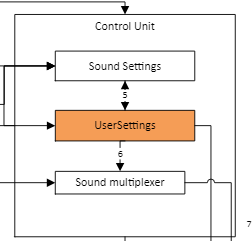
\includegraphics[width=0.60\textwidth]{images/UserSettings}
 \caption{User Settings subsystem description diagram}
\end{figure}


\subsubsection{Assumptions}
\begin{itemize}
\begin{item}
The UserSettings subsystem receives digital signals from the Sound Settings subsystem 
\end{item}
\begin{item}
The UserSettings subsystem can receive user input from the Input Layer subsystems
\end{item}
\begin{item}
The UserSettings subsystem is responsible for managing and updating the user's settings
\end{item}
\end{itemize}
\subsubsection{Responsibilities}
\begin{itemize}
\begin{item}
Receive user input from the Input Layer subsystems.
\end{item}
\begin{item}
Process and validate user input.
\end{item}
\begin{item}
Update the user's settings based on the validated input.
\end{item}
\begin{item}
Send digital signals representing the user's settings to the Sound Settings subsystem
\end{item}
\end{itemize}

\subsubsection{Subsystem Interfaces}
\begin {table}[H]
\caption {Subsystem interfaces} 
\begin{center}
    \begin{tabular}{ | p{1cm} | p{6cm} | p{3cm} | p{3cm} |}
    \hline
    ID & Description & Inputs & Outputs \\ \hline
    \#1 & Receives digital signals from the Sound Settings & \pbox{3cm}{ \\ Digital signals representing sound settings } & \pbox{3cm}{Touchscreen}  \\ \hline
    
    \end{tabular}
\end{center}
\end{table}
\subsection{Sound multiplexer}
The Sound Multiplexer subsystem is connected to the Sound Settings subsystem and the Output Layer
\begin{figure}[h!]
	\centering
 	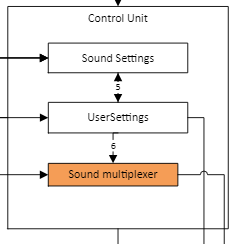
\includegraphics[width=0.60\textwidth]{images/Soundmultiplex}
 \caption{Sound Multiplexer subsystem description diagram}
\end{figure}


\subsubsection{ASSUMPTIONS}
\begin{itemize}
\begin{item}
The Sound Multiplexer subsystem receives digital signals from the Sound Settings subsystem 
\end{item}
\begin{item}
The Sound Multiplexer subsystem can select and output the appropriate sound based on the received settings.
\end{item}
\begin{item}
The Sound Multiplexer subsystem is responsible for managing and outputting the final sound signal.
\end{item}
\end{itemize}
\subsubsection{SUBSYSTEM INTERFACES}
\begin {table}[H]
\caption {Subsystem interfaces} 
\begin{center}
    \begin{tabular}{ | p{1cm} | p{6cm} | p{3cm} | p{3cm} |}
    \hline
    ID & Description & Inputs & Outputs \\ \hline
    \#1 & Representing the desired sound settings from the Sound Settings subsystem & \pbox{3cm}{ \\ User settings and input } & \pbox{3cm}{Speaker}  \\ \hline
  
    \end{tabular}
\end{center}
\end{table}